\section{Special case: Limited resolution}
\label{sec:empirical}

As Le et al. proved in~\cite{Le2013}, we only need consider interval
start times as candidate splitters.  Many datasets have the number of
candidate splitters, i.e. distinct interval start times, that is
orders of magnitude smaller than N. This is due to the fact that time
is of limited granularity and in many cases updates come in
batches. \vera{need some empirical data here on several temporal
  datasets}

We define $L$ as the set of candidate splitters:

$L = \{l, [s_i,e_i] \in I | l = s_i\}$

$|L| = m$

When $m << N$, we can define an algorithm that uses m-size index
rather than N-sized stabbing count array.  Similar to Le, we define
$I^-(l)$ and $I^e(l)$ as the subsets of intervals of I whose starting
values are less than $l$ and ending values are less than $l$,
respectively:

$I^-(l) = \{[s_i,e_i] \in I | s_i < l\}$

$I^e(l) = \{[s_i,e_i] \in I | e_i < l\}$

In other words, $I^-(l)$ contains all the intervals that have started
before $l$ and $I^e(l)$ all the intervals that have ended before $l$.
By definition, $I^e(l) \in I^-(l)$.

For each $j \in [1, m]$, we define $s[j]$ as the number of intervals
that have started before $l_j$, and $e[j]$ as the number of intervals
that have ended before $l_j$, i.e.,

$s[j] = |I^-(l_j)|$

$e[j] = |I^e(l_j)|$

The start index is an array of size $m$ where $A[j] = (l_j, s[j],
e[j])$, $1 \leq j \leq m$.  Figure~\ref{fig:startindex} shows the
start index for the intervals in Figure~\ref{fig:stabarray}.  Note
that in this example $m = 7$ which is not significantly smaller than
$n = 9$, so it is not a scenario where this approach would be
beneficial.

\begin{figure}
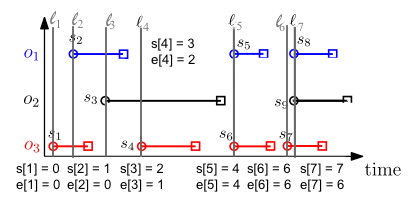
\includegraphics[width=3in]{figs/startindex.png}
\caption{Start index.}
\label{fig:startindex}
\end{figure}

We can calculate the start index with the following SQL commands:

\begin{small}
\begin{verbatim}
select L.s, count(*)
from I, (select distinct s from I) as L
where I.s < L.s
group by L.s
order by L.s

select L.s, count(*)
from I, (select distinct s from I) as L
where I.e < L.s
group by L.s
order by L.s
\end{verbatim}
\end{small}

In a distributed system we can efficiently calculate the start index
by using a single broadcast join of $I$ with a much smaller $L$.  As
an additional performance improvement, we can avoid $m*N$ increase in
output during the join by joining each interval in I with the smallest
$l$ that meets the selection criteria, followed by group by, sort, and
scan left to get the totals.

To construct the start index, we use $W(N) = \Theta(N) + 2\Theta(m*N)
+ \Theta(m~log~m) = O(mN)$, $S(N) = \Theta(1) + \Theta(log~mN) +
\Theta(log^2 m) = O(log~N)$.

Given the start index A, we can traverse it from smallest to largest,
taking up to $t$ intervals greedily in $O(m)$ time for a single
traversal.  As in the original t-jump, the algorithm outputs
$\overline{t}$ and a partition $P$ with splitters $l_1, \ldots, l_k$,
where $k$ is some integer between 0 and $k$, such that $c(P) =
\overline{t} \leq t$.  To find the smallest $t$ that yields a valid
partition, we use binary search.  As in the baseline approach, with a
concurrent search of $h$ candidate $t$s, $W(n) = \Theta(log_hN*hm)$,
$S(n) = \Theta(log_hN)$.

Thus in a special case where $m << N$, we can solve the optimal
splitters problem in $O(mN)$, which is more efficient than the
baseline $O(N~log~N)$ as long as $m < log N$.  This approach has the
additional benefit that the start index is small enough to fit into
internal memory even for very large values of $N$, unlike the stabbing
count array.
